\subsection{Entropía}\label{entropuxeda}

\subsubsection{Preliminares}\label{preliminares}

\paragraph{Variable aleatoria}\label{variable-aleatoria}

Una variable aleatoria es una función que asigna un valor numérico a
cada resultado de un experimento aleatorio. Por ejemplo, si lanzamos un
dado, la variable aleatoria \(X\) que representa el número que sale en
la cara superior del dado, puede tomar los valores \(1, 2, 3, 4, 5, 6\).
En ese caso escribiríamos que

\[
X = \{1,2,3,4,5,6\}
\]

Osea, \(X\) es una variable aleatoria que toma valores en el conjunto
\(\{1,2,3,4,5,6\}\).

En el ejemplo anterior, la variable aleatoria \(X\) es discreta, porque
toma valores en un conjunto finito o numerable (recuerda, hay infinitos
más grandes que otros. Un infinito numerable es aquel que se puede poner
en correspondencia con los números naturales \(\mathbb{N}\)). Pero
también hay variables aleatorias continuas, que toman valores en un
intervalo de números reales. Por ejemplo, si medimos la altura de una
persona, la variable aleatoria que representa la altura puede tomar
cualquier valor en el intervalo \((0,\infty)\).

\paragraph{Función de probabilidad}\label{funciuxf3n-de-probabilidad}

La función de probabilidad de una variable aleatoria es una función que
asigna a cada valor de la variable aleatoria la probabilidad de que ese
valor ocurra. Por ejemplo, si lanzamos un dado, la función de
probabilidad de la variable aleatoria \(X\) que representa el número que
sale en la cara superior del dado, es una función que asigna a cada
número del conjunto \(\{1,2,3,4,5,6\}\) la probabilidad de que salga ese
número. En este caso, la función de probabilidad es uniforme, porque
todos los números tienen la misma probabilidad de salir.

Para una variable aleatoria discreta, la función de probabilidad se
puede representar mediante una tabla o mediante una fórmula. Por
ejemplo, si lanzamos un dado, la función de probabilidad de la variable
aleatoria \(X\) que representa el número que sale en la cara superior
del dado, se puede representar mediante la siguiente tabla:

\begin{longtable}[]{@{}ll@{}}
\toprule\noalign{}
\(x\) & \(P(X=x)\) \\
\midrule\noalign{}
\endhead
\bottomrule\noalign{}
\endlastfoot
1 & 1/6 \\
2 & 1/6 \\
3 & 1/6 \\
4 & 1/6 \\
5 & 1/6 \\
6 & 1/6 \\
\end{longtable}

O mediante la siguiente fórmula:

\[
P(X=x) = \frac{1}{6} \quad \text{para } x \in \{1,2,3,4,5,6\}
\]

Para una variable aleatoria continua, la función de probabilidad se
puede representar mediante una función de densidad de probabilidad. Por
ejemplo, si medimos la altura de una persona, la función de densidad de
probabilidad de la variable aleatoria que representa la altura, es una
función que asigna a cada valor del intervalo \((0,\infty)\) la
probabilidad de que la altura de una persona esté en ese intervalo.

\paragraph{Esperanza matemática}\label{esperanza-matemuxe1tica}

La esperanza matemática de una variable aleatoria es el valor promedio
que toma la variable aleatoria en un experimento aleatorio. Se calcula
multiplicando cada valor de la variable aleatoria por su probabilidad, y
sumando los resultados:

\[
\mathbb{E}[X] = \sum_{i=0}^n x_i \cdot P(X=x_i)
\]

Por ejemplo, si lanzamos un dado, la esperanza matemática de la variable
aleatoria \(X\) que representa el número que sale en la cara superior
del dado, se calcula como

\[
\mathbb{E}[X] = 1 \cdot \frac{1}{6} + 2 \cdot \frac{1}{6} + 3 \cdot \frac{1}{6} + 4 \cdot \frac{1}{6} + 5 \cdot \frac{1}{6} + 6 \cdot \frac{1}{6} = 3.5
\]

Osea, en promedio, el número que sale en la cara superior del dado es
3.5.

Para una variable aleatoria continua, la esperanza matemática se calcula
de forma similar, pero en lugar de sumar los valores de la variable
aleatoria, se integran:

\[
\mathbb{E}[X] = \int_{-\infty}^{\infty} xf(x)dx
\]

Donde \(f(x)\) es la función de densidad de probabilidad de la variable
aleatoria \(X\).

\paragraph{\texorpdfstring{LOTUS: \emph{Law of the Unconscious
Statistician} (Ley del Estadístico
Inconsciente)}{LOTUS: Law of the Unconscious Statistician (Ley del Estadístico Inconsciente)}}\label{lotus-law-of-the-unconscious-statistician-ley-del-estaduxedstico-inconsciente}

La LOTUS es una regla que permite calcular la esperanza matemática de
una función de una variable aleatoria, sin necesidad de conocer la
función de probabilidad de la variable aleatoria. La LOTUS establece que
la esperanza matemática de una función de una variable aleatoria se
calcula multiplicando la función por la función de probabilidad de la
variable aleatoria, y sumando los resultados:

\[
\mathbb{E}[g(X)] = \sum_{i=0}^n g(x_i) \cdot P(X=x_i)
\]

Por ejemplo, si lanzamos un dado, y definimos la variable aleatoria
\(Y = X^2\), donde \(X\) es la variable aleatoria que representa el
número que sale en la cara superior del dado, la esperanza matemática de
la variable aleatoria \(Y\) se calcula como

\[
\mathbb{E}[Y] = 1^2 \cdot \frac{1}{6} + 2^2 \cdot \frac{1}{6} + 3^2 \cdot \frac{1}{6} + 4^2 \cdot \frac{1}{6} + 5^2 \cdot \frac{1}{6} + 6^2 \cdot \frac{1}{6} = 15.1667
\]

Osea, en promedio, el cuadrado del número que sale en la cara superior
del dado es 15.1667.

Para una variable aleatoria continua, la LOTUS se calcula de forma
similar, pero en lugar de sumar los valores de la variable aleatoria, se
integran:

\[
\mathbb{E}[g(X)] = \int_{-\infty}^{\infty} g(x)f(x)dx
\]

Donde \(f(x)\) es la función de densidad de probabilidad de la variable
aleatoria \(X\).

\subsubsection{Entropía}\label{entropuxeda-1}

En física, la entropía es una medida de la cantidad de desorden o caos
en un sistema; más concretamente en termodinámica, la entropía es una
medida de la cantidad de energía que no se puede utilizar para realizar
trabajo. En teoría de la información, la entropía es una medida de la
incertidumbre de una variable aleatoria. También se puede interpretar
como una medida de la cantidad de información que se necesita para
describir una variable aleatoria.

La entropía de una variable aleatoria \(X\) se define como la esperanza
matemática de la información de la variable aleatoria. La información de
una variable aleatoria es una medida de la ``\emph{sorpresa}'' que
produce un valor de la variable aleatoria.

La información de una variable aleatoria se calcula como el negativo del
logaritmo de la probabilidad de que ocurra un valor de la variable
aleatoria:

\[
I(x) = -\log_n\left(P(X=x)\right)
\]

Nótese que la base del logaritmo determina la unidad de medida de la
información. Esta base puede ser cualquier número positivo, pero las
bases más comunes son:

\begin{itemize}
\tightlist
\item
  \texttt{2}: en cuyo caso la unidad de medida de la información es el
  \emph{bit} (binary digit).
\item
  \texttt{e}: en cuyo caso la unidad de medida de la información es el
  \emph{nat} (natural unit of information).
\item
  \texttt{10}: en cuyo caso la unidad de medida de la información es el
  \emph{hartley}.
\end{itemize}

\textbf{En caso de no especificar ninguna base, asumiremos que la base
del logaritmo es 2.}

Sabiendo esto, la entropía de una variable aleatoria \(X\), que
denotaremos como \(H_k(X)\), se calcula de la siguiente manera (gracias
al teorema LOTUS):

\[
H_k(X) = \mathbb{E}[I(X)] = \sum_{i=0}^n -\log_k\left(P(X=x_i)\right) \cdot P(X=x_i)
\]

O para una variable aleatoria continua:

\[
H_k(X) = \int_{-\infty}^{\infty} -\log_k\left(f(x)\right) \cdot f(x)dx
\]

donde el subíndice \(k\) indica la base del logaritmo. \textbf{Recordad
que si no se especifica ninguna base, asumiremos que la base del
logaritmo es 2.}

En teoría de la información, partiremos de una fuente de información
definida como un par \((S,P)\) donde \(S\) es un alfabeto predefinido y
\(P\) es una distribución de probabilidad sobre \(S\).

Dado que la fuente de información introduce una incertidumbre en la
variable aleatoria definida por el alfabeto predefinido, la entropía nos
será de utilidad para medir el grado de incertidumbre, el grado de
aleatoriedad en la fuente de información y, en consecuencia, estimar las
unidades de información necesarias en promedio para codificar todos los
valores posibles que puedan darse en la fuente de información.

Debido a las propiedades del logaritmo, \(H_k(X)\) admite las siguientes
definiciones alternativas (pero equivalentes):

\begin{itemize}
\tightlist
\item
  \(H_k(X) = -\sum_{i=0}^n\log_k\left(P(X=x_i)\right)\cdot P(X=x_i)\)
\item
  \(H_k(X) = \sum_{i=0}^n \log_k\left(\frac{1}{P(X=x_i)}\right)P(X=x_i)\)
\end{itemize}

Además, debido a las propiedades del logaritmo (en particular que
\(\log_a(b)=\frac{\log_c(b)}{\log_c(a)}\)), se cumple que
\(H_b(X)=\log_b(a)\cdot H_a(X)\). La demostración es sencilla:


\begin{align*}
H_b(X) &= \sum_{i=0}^n -\log_b\left(P(X=x_i)\right) \cdot P(X=x_i) \\
&= \sum_{i=0}^n -\frac{\log_a\left(P(X=x_i)\right)}{\log_a(b)} \cdot P(X=x_i) \\
&= \frac{1}{\log_a(b)}\sum_{i=0}^n -\log_a\left(P(X=x_i)\right) \cdot P(X=x_i) \\
&= \left(\frac{1}{\log_a(b)}\right)H_a(X) \\
&= \left(\frac{1}{\frac{\log_b(b)}{\log_b(a)}}\right)H_a(X) \\
&= \left(\frac{1}{\frac{1}{\log_b(a)}}\right)H_a(X) \\
&= \log_b(a)\cdot H_a(X) \\
\end{align*}

\begin{center}\rule{0.5\linewidth}{0.5pt}\end{center}

\paragraph{Ejemplo 1: Entropía de una variable aleatoria
discreta}\label{ejemplo-1-entropuxeda-de-una-variable-aleatoria-discreta}

\emph{Sea el alfabeto \(S=\left\{a,b,c,d\right\}\) con una distribución
de probabilidades
\(P=\left\{\frac{1}{2},\frac{1}{4},\frac{1}{8},\frac{1}{8}\right\}\). La
entropía de la variable aleatoria \(X\) definida por el alfabeto \(S\) y
la distribución de probabilidad \(P\) es:}

\[
H(X) = -\left(\frac{1}{2}\log\left(\frac{1}{2}\right) + \frac{1}{4}\log\left(\frac{1}{4}\right) + \frac{1}{8}\log\left(\frac{1}{8}\right) + \frac{1}{8}\log\left(\frac{1}{8}\right)\right) = 1.75
\]

La entropia de la variable aleatoria \(X\) es 1.75 bits.

\begin{center}\rule{0.5\linewidth}{0.5pt}\end{center}

Una propiedad interesante de la entropía es la siguiente: sea \(X\) una
variable aleatoria sobre el alfabeto
\(\left\{x_1,x_2,\dots,x_n\right\}\), entonces:

\[
0 \leq H(X) \leq \log(n)
\]

La entropía de una variable aleatoria \(X\) está acotada por \(0\) y
\(\log(n)\), donde \(n\) es el número de elementos del alfabeto de la
variable aleatoria. La entropía es máxima cuando la distribución de
probabilidad es uniforme, y es mínima cuando la distribución de
probabilidad es degenerada (es decir, cuando un único valor del alfabeto
tiene probabilidad 1 y el resto de valores tienen probabilidad 0).

\begin{center}\rule{0.5\linewidth}{0.5pt}\end{center}

\paragraph{Ejemplo 2: Entropía de una variable aleatoria distribuida
bernoulli}\label{ejemplo-2-entropuxeda-de-una-variable-aleatoria-distribuida-bernoulli}

\emph{Sea \(X\) una variable aleatoria distribuida Bernoulli con
parámetro \(p\) (es decir, \(X\sim\text{Bernoulli}(p)\), lo cual quiere
decir que nuestra variable aleatoria mide ``el número de éxitos en un
experimento de Bernoulli''). La función de probabilidad de \(X\) es:}

\[
P(X=x) = p^x(1-p)^{1-x} \quad \text{para } x\in\{0,1\}
\]

\emph{La entropía de la variable aleatoria \(X\) es:}


\begin{align*}
H(X) &= -\sum_{x=0}^1 p^x(1-p)^{1-x}\log\left(p^x(1-p)^{1-x}\right) \\
&= -\left(p\log(p) + (1-p)\log(1-p)\right) \\
&= (p-1)\log(1-p) -p\log(p)
\end{align*}

Si representamos la entropía de la variable aleatoria \(X\) en función
de \(p\), obtenemos la siguiente gráfica:

\begin{figure}[htbp!]
\centering
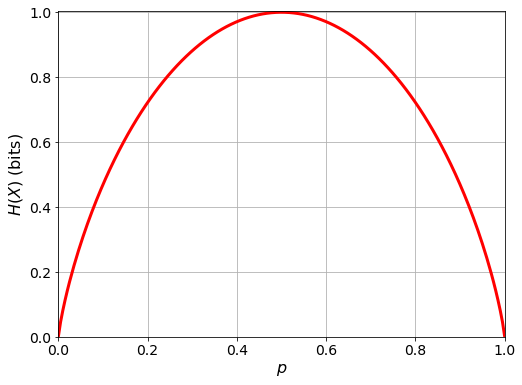
\includegraphics[width=0.95\linewidth]{./img/bernoulli_entropy.png}
\end{figure}

\emph{¿Qué interpretación tiene esto?} La entropía de una variable
aleatoria Bernoulli es máxima cuando \(p=0.5\), es decir, cuando la
distribución de probabilidad es uniforme. Esto tiene sentido, porque en
una distribución uniforme, todos los valores del alfabeto tienen la
misma probabilidad de ocurrir, y por lo tanto hay más incertidumbre
sobre el valor que tomará la variable aleatoria. Por otro lado, la
entropía de una variable aleatoria Bernoulli es mínima cuando \(p=0\) o
\(p=1\), es decir, cuando la distribución de probabilidad es degenerada.
Esto también tiene sentido, porque en una distribución degenerada, solo
un valor del alfabeto tiene probabilidad 1 y el resto de valores tienen
probabilidad 0, y por lo tanto no hay incertidumbre sobre el valor que
tomará la variable aleatoria.

\emph{¿Cómo se programaría esto en \texttt{python}?}

\begin{Shaded}
\begin{Highlighting}[]
\ImportTok{import}\NormalTok{ numpy }\ImportTok{as}\NormalTok{ np}
\ImportTok{import}\NormalTok{ matplotlib.pyplot }\ImportTok{as}\NormalTok{ plt}

\KeywordTok{def}\NormalTok{ H\_Bernoulli(p):}

\NormalTok{    h }\OperatorTok{=}\NormalTok{ (p }\OperatorTok{{-}} \DecValTok{1}\NormalTok{)}\OperatorTok{*}\NormalTok{np.log2(}\DecValTok{1} \OperatorTok{{-}}\NormalTok{ p) }\OperatorTok{{-}}\NormalTok{ p}\OperatorTok{*}\NormalTok{np.log2(p)}
    
    \CommentTok{\# Fix the NaN values that occur due to the logarithm of zero}
\NormalTok{    h[np.isnan(h)] }\OperatorTok{=} \DecValTok{0}

    \ControlFlowTok{return}\NormalTok{ h}

\NormalTok{plt.figure(figsize}\OperatorTok{=}\NormalTok{(}\DecValTok{8}\NormalTok{, }\DecValTok{6}\NormalTok{))}

\NormalTok{p }\OperatorTok{=}\NormalTok{ np.linspace(}\DecValTok{0}\NormalTok{, }\DecValTok{1}\NormalTok{, }\DecValTok{200}\NormalTok{)}
\NormalTok{plt.plot(p, H\_Bernoulli(p), }\StringTok{"r"}\NormalTok{, linewidth}\OperatorTok{=}\DecValTok{3}\NormalTok{)}

\NormalTok{plt.grid()}
\NormalTok{plt.xlim(}\DecValTok{0}\NormalTok{, }\DecValTok{1}\NormalTok{)}
\NormalTok{plt.ylim(}\DecValTok{0}\NormalTok{, }\FloatTok{1.005}\NormalTok{)}
\NormalTok{plt.ylabel(}\VerbatimStringTok{r"$H(X)$ (bits)"}\NormalTok{, fontsize}\OperatorTok{=}\DecValTok{16}\NormalTok{)}
\NormalTok{plt.xlabel(}\VerbatimStringTok{r"$p$"}\NormalTok{, fontsize}\OperatorTok{=}\DecValTok{16}\NormalTok{)}
\NormalTok{plt.tick\_params(axis}\OperatorTok{=}\StringTok{"both"}\NormalTok{, which}\OperatorTok{=}\StringTok{"major"}\NormalTok{, labelsize}\OperatorTok{=}\DecValTok{14}\NormalTok{)}
\end{Highlighting}
\end{Shaded}

\paragraph{Recordatorio: probabilidades conjuntas y
condicionales}\label{recordatorio-probabilidades-conjuntas-y-condicionales}

Dadas dos variables aleatorias \(X\) e \(Y\), la probabilidad conjunta
de \(X\) e \(Y\) es la probabilidad de que ambas variables aleatorias
tomen un valor determinado. Se denota como \(P(X=x,Y=y)\), y se calcula
de la siguiente manera:

\[
P(X=x,Y=y) = P(Y=y|X=x)P(X=x)
\]

donde \(P(Y=y|X=x)\) es la probabilidad condicional de \(Y\) dado \(X\),
es decir, la probabilidad de que \(Y\) tome un valor determinado dado
que \(X\) ha tomado un valor determinado.

De la misma manera, podemos definir la probabilidad conjunta como

\[
P(X=x,Y=y) = P(X=x|Y=y)P(Y=y)
\]

Igualando ambas expresiones, se obtiene el Teorema de Bayes:

\[
P(Y=y|X=x) = \frac{P(X=x|Y=y)P(Y=y)}{P(X=x)}
\]

Además, si las variables aleatorias \(X\) e \(Y\) son independientes,
entonces la probabilidad conjunta de \(X\) e \(Y\) es igual al producto
de las probabilidades marginales de \(X\) e \(Y\):

\[
P(X=x,Y=y) = P(X=x)P(Y=y)
\]

¿Por qué? Porque si \(X\) e \(Y\) son independientes, entonces la
probabilidad de que \(Y\) tome un valor determinado no depende de que
\(X\) haya tomado un valor determinado, y viceversa, por ende
\(P(Y=y|X=x) = P(Y=y)\) y \(P(X=x|Y=y) = P(X=x)\).

\paragraph{Entropía conjunta y entropía
condicional}\label{entropuxeda-conjunta-y-entropuxeda-condicional}

Hasta ahora hemos definido la entropía de una única variable aleatoria.
Pero en muchos problemas de teoría de la información, estamos
interesados en la entropía de dos o más variables aleatorias.

La entropía conjunta de dos variables aleatorias \(X\) e \(Y\) se define
como la entropía de la variable aleatoria \((X,Y)\), que es una variable
aleatoria que toma valores en el producto cartesiano (es decir, todas
las parejas posibles) de los alfabetos de \(X\) e \(Y\). La entropía
conjunta de \(X\) e \(Y\) se denota como \(H(X,Y)\), y se calcula de la
siguiente manera:

\[
H(X,Y) = -\sum_{x\in S_X}\sum_{y\in S_Y} P(X=x,Y=y)\log\left(P(X=x,Y=y)\right)
\]

O para variables aleatorias continuas:

\[
H(X,Y) = -\int_{-\infty}^{\infty}\int_{-\infty}^{\infty} f(x,y)\log\left(f(x,y)\right)dxdy
\]

Otra manera de escribir la entropía conjunta sería utilizando índices
para los valores de las variables aleatorias:

\[
H(X,Y) = -\sum_{i=0}^n\sum_{j=0}^m P(X=x_i,Y=y_j)\log\left(P(X=x_i,Y=y_j)\right)
\]

En algunos casos, esta notación es más clara que la notación con los
alfabetos \(S_X\) y \(S_Y\). Habitualmente \(S_X = S_Y\), es decir,
estamos usando el mismo alfabeto para ambas variables aleatorias.

De forma similar a la entropía conjunta, podemos definir la entropía
condicional de una variable aleatoria \(X\) dada otra variable aleatoria
\(Y\). La entropía condicional de \(X\) dado \(Y\) se denota como
\(H(X|Y)\), y se calcula de la siguiente manera:

\[
H(X|Y) = -\sum_{x\in S_X}\sum_{y\in S_Y} P(X=x,Y=y)\log\left(P(X=x|Y=y)\right)
\]

Es más, utilizando las propiedades de las probabilidades conjuntas y
condicionales, podemos escribir la entropía condicional de \(X\) dado
\(Y\) de la siguiente manera:


\begin{align*}
H(X|Y) &= -\sum_{x\in S_X}\sum_{y\in S_Y} P(X=x,Y=y)\log\left(P(X=x|Y=y)\right) \\
&= -\sum_{x\in S_X}\sum_{y\in S_Y} P(X=x|Y=y)P(Y=y)\log\left(P(X=x|Y=y)\right) \\
&= -\sum_{y\in S_Y} P(Y=y)\sum_{x\in S_X} P(X=x|Y=y)\log\left(P(X=x|Y=y)\right) \\
&= \sum_{y\in S_Y} P(Y=y)H(X|Y=y)
\end{align*}


De la misma manera que hemos hecho en la demostración anterior, las
propiedades de la entropia conjunta se originan de operar con las
probabilidades conjuntas y condicionales de las variables aleatorias
\(X\) e \(Y\).

Una de estas propiedades es

\[
H(X,Y) = H(X) + H(Y|X) = H(Y) + H(X|Y)
\]

Esta propiedad se conoce como la regla de la cadena de la entropía, y se
puede demostrar a partir de la definición de la entropía conjunta y
condicional:

\begin{align*}
H(X,Y) &= -\sum_{x\in S_X}\sum_{y\in S_Y} P(X=x,Y=y)\log\left(P(X=x,Y=y)\right) \\
&= -\sum_{x\in S_X}\sum_{y\in S_Y} P(X=x,Y=y)\log\left(P(X=x|Y=y)P(Y=y)\right) \\
&= -\sum_{x\in S_X}\sum_{y\in S_Y} P(X=x,Y=y)\left(\log\left(P(X=x|Y=y)\right) + \log\left(P(Y=y)\right)\right) \\
&= -\sum_{x\in S_X}\sum_{y\in S_Y} P(X=x,Y=y)\log\left(P(X=x|Y=y)\right) - \sum_{x\in S_X}\sum_{y\in S_Y} P(X=x,Y=y)\log\left(P(Y=y)\right) \\
&= H(X|Y) - \sum_{y\in S_Y} P(Y=y)\log\left(P(Y=y)\right) \\
&= H(X|Y) + H(Y)
\end{align*}


De la misma manera, se puede demostrar que \(H(X,Y) = H(Y) + H(X|Y)\).

De este resultado se puede demostrar que dadas las variables aleatorias
\(X\) e \(Y\):

\begin{enumerate}
\def\labelenumi{\arabic{enumi}.}
\tightlist
\item
  \(H(X,Y) \leq H(X) + H(Y)\)
\item
  \(H(X,Y) = H(X) + H(Y)\), (en caso de que \(X\) e \(Y\) sean
  independientes)
\end{enumerate}

\emph{Una forma sencilla de pensar sobre estas propiedades es pensar en
las probabilidades conjuntas y condicionales, de las cuales obtenemos
desigualdades similares, solamente que en el caso de la entropía, debido
al logaritmo, las desigualdades no son productos si no sumas.}

Un corolario de las propiedades anteriores es que:

\begin{enumerate}
\def\labelenumi{\arabic{enumi}.}
\tightlist
\item
  \(H(X|Y) \leq H(X)\)
\item
  \(H(X|Y) = H(X)\), (en caso de que \(X\) e \(Y\) sean independientes)
\end{enumerate}

\begin{center}\rule{0.5\linewidth}{0.5pt}\end{center}

Volviendo a la regla de la cadena, esta la podemos extender para el caso
de más de dos variables, y se define como:

\[
H(X_1,X_2,\dots,X_n) = H(X_1) + H(X_2|X_1) + H(X_3|X_1,X_2) + \dots + H(X_n|X_1,X_2,\dots,X_{n-1})
\]

o de forma más compacta:

\[
H(X_1,X_2,\dots,X_n) = \sum_{i=1}^n H(X_i|X_1,X_2,\dots,X_{i-1})
\]

\paragraph{Entropía Relativa}\label{entropuxeda-relativa}

La entropía relativa, también conocida como divergencia de
Kullback-Leibler, es una medida de la diferencia entre dos
distribuciones de probabilidad (la cantidad de información que se
necesita para describir una distribución de probabilidad utilizando otra
distribución de probabilidad). La entropía relativa de dos
distribuciones de probabilidad \(P\) y \(Q\) se denota como \(D(P||Q)\),
y se calcula de la siguiente manera:

\[
D(P||Q) = \sum_{x\in S} P(x)\log\left(\frac{P(x)}{Q(x)}\right)
\]

O para distribuciones de probabilidad continuas:

\[
D(P||Q) = \int_{-\infty}^{\infty} f(x)\log\left(\frac{f(x)}{g(x)}\right)dx
\]

La entropía relativa es siempre \textbf{no negativa}, y es igual a cero
si y solo si \(P\) y \(Q\) son iguales.

\paragraph{Información Mutua}\label{informaciuxf3n-mutua}

La información mutua de dos variables aleatorias \(X\) e \(Y\) es una
medida de la cantidad de información que una variable aleatoria
proporciona sobre la otra variable aleatoria. La información mutua de
\(X\) e \(Y\) se denota como \(I(X;Y)\), y se calcula de la siguiente
manera:

\[
I(X;Y) = \sum_{x\in S_X}\sum_{y\in S_Y} P(X=x,Y=y)\log\left(\frac{P(X=x,Y=y)}{P(X=x)P(Y=y)}\right)
\]

O para variables aleatorias continuas:

\[
I(X;Y) = \int_{-\infty}^{\infty}\int_{-\infty}^{\infty} f(x,y)\log\left(\frac{f(x,y)}{f(x)f(y)}\right)dxdy
\]

La información mutua es siempre \textbf{no negativa}, y es igual a cero
si y solo si \(X\) e \(Y\) son independientes. Se puede pensar también
que la información mutua es la entropía relativa entre la distribución
conjunta de dos variables aleatorias y el producto de sus distribuciones
marginales.

De la definición de la información mutua se pueden deducir las
siguientes propiedades:

\begin{enumerate}
\def\labelenumi{\arabic{enumi}.}
\tightlist
\item
  \(I(X;Y) = H(X) - H(X|Y) = H(Y) - H(Y|X)\)
\item
  \(I(X;Y) = H(X) + H(Y) - H(X,Y)\)
\item
  \(I(X;Y) = I(Y;X)\)
\item
  \(I(X;X) = H(X)\)
\end{enumerate}

Gráficamente, estas propiedades se pueden representar de la siguiente
manera:
\vspace{-9cm}
\begin{figure}[htbp!]
\centering
\includesvg[width=\linewidth]{./img/mutual_information_relation_diagram.svg}
\end{figure}
